\subsection{Across experiments: what decides a life}

Experiments 1-4 used different judges. Here we pool their 14-day WebShop lives (1-A, 1-C, 2, 3 with its sleep variant, and 4) and ask what predicts where a life ends. It was the share of its lessons that were failed attempts, not the number of lessons or the kind of judge.

\begin{figure}[htbp]
\centering
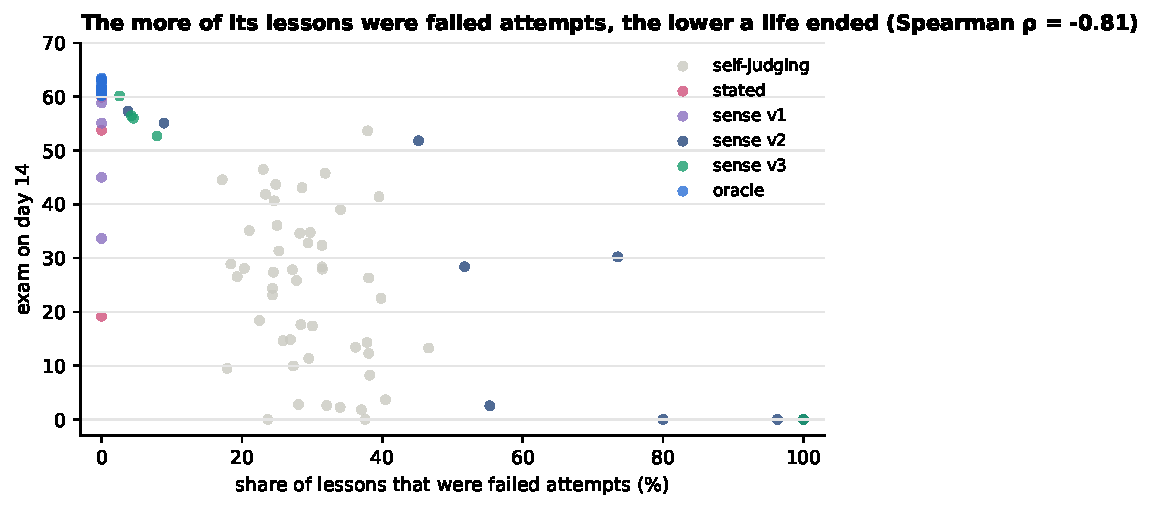
\includegraphics[width=1.0\linewidth]{figures/fig6_failed_lessons}
\caption{All 14-day WebShop lives in Experiments 1-4, including 1-C, that learned at least once (97 of 104); lessons counted to day 14; Exp 3b = the sleep variant of Experiment 3}
\label{fig:6}
\end{figure}

Across 97 lives, the share of failed attempts among a life's lessons in its first 14 days predicted its day-14 exam closely (Spearman $\rho$ = -0.81, p \textless{} 0.001). The \emph{oracle} lives, all at 0\% failures and about 63, do not drive this alone: among the 72 lives not judged by the \emph{oracle}, $\rho$ = -0.61 (p \textless{} 0.001). Every \emph{oracle} life learned only from successes and ended at 60-63. Self-judging lives let in 17-47\% failures and ended anywhere from 0 to 54. The sense lives, all three versions together, split cleanly: the ten that let in under 10\% failures ended at 34-60; the nine that let in 45\% or more ended at 0-52, six of them at 0-3. Experiment 5 fits the same pattern, although it stays out of the statistic because its scores are on another scale: the \emph{sense v3} lives learned from 80\% failed attempts, and the 1.7B lives collapsed.

The number of lessons mattered less than we expected. In Experiment 2 the \emph{sense v1} lives learned from only 0-7 lessons in 14 days and still reached 34-59; in Experiment 1, the \emph{stated verdict} learned from 0-7, none of them failures, and reached up to 61. A few correct lessons are enough to teach the shop's basic routine, and a few wrong ones are enough to undo it.

This explains why a single bad night can end a sense life. A sense life learned from only 0-6 lessons on night 1, so one failed attempt could be most of its first night's training. Of the 20 sense lives in Experiments 2-4 (v1 in Experiment 2, v2 in Experiment 3, v3 in Experiment 4), seven learned from a failed attempt on night 1, and six of those seven ended at 0-3 (Fisher exact test, p \textless{} 0.001). Of the thirteen without one, none ended below 28, except one that never learned anything at all (6).
